\chapter{Especificações e Arquitetura do Sistema}
\label{chap:arquitetura}
Durante todo o desenvolvimento do sistema, buscou-se não se utilizar dos modelos de arquitetura comumente empregados neste tipo de aplicação, que trabalham com grandes volumes de dados, um dos motivos vem a ser pela grande complexidade encontrada ao se trabalhar com módulos Apache como o Hadoop Common, Hadoop Distributed File System (HDFS), Hadoop YARN e Hadoop MapReduce, os quais dependendo de suas aplicações acabam por gerar dependências de outras ferramentas como Cassandra, Spark, ZooKeeper, entre outras que se mostram apesar de robustas, muito complexas e com uma curva de aprendizagem alta demais para serem usadas de imediato.

Outro motivo de grande valor para o desenvolvimento de uma nova arquitetura tem sido a empregabilidade de novas ferramentas utilizadas no lado \textit{backend}, por assim dizer, relacionado a organização dentro dos servidores, conceitos de desenvolvimento e bancos de dados que tem ganhado força dentro do mercado e se mostradas bem aplicáveis em projetos com grandes volumes de dados e alta disponibilidade, além de possuir uma baixa curva de aprendizagem, se comparadas com as tecnologias tradicionais.

\section{Docker}
\label{sec:docker}
O Docker é uma plataforma aberta criada com o intuito de tornar mais ágil o desenvolvimento, implantação e execução de aplicações em ambientes isolados, além de ser multiplataforma, tudo isso através do conceito de conteinerização e imagens, em que numa imagem se tem todos os arquivos necessários para a criação de um contêiner, este por sua vez, possui a aplicação encapsulada  e funcionando.

Desta forma se tem uma grande flexibilidade para trabalhar com as aplicações, pois estas irão funcionar tanto em um notebook, quanto em um mainframe. Este conceito de contêiner se assimila ao processo de criação de máquinas virtuais, onde se tem todo o sistema operacional virtualizado, já o Docker realiza uma virtualização á nível do sistema operacional, mantendo um único kernel no \textit{host} executando processos (contêineres) de forma isolada, isso é possível através do uso de \textit{namespaces}, fazendo com que um processo só tenha acesso a recursos de outro se isso for explicitamente configurado na criação dos ambientes. Para que não ocorra a exaustão de recursos no \textit{host} o Docker se utiliza de \textit{cgroups} do kernel, responsável por criar limites de hardware para os processos, evitando o uso exagerado de recursos por apenas um processo. A figura \ref{fig:arqdocker} apresenta a organização a nível de sistema operacional de um \textit{host} utilizando Docker.~\cite{docker}

\begin{figure}[!h]
\caption{\label{fig:arqdocker} Arquitetura Docker}
\begin{center}
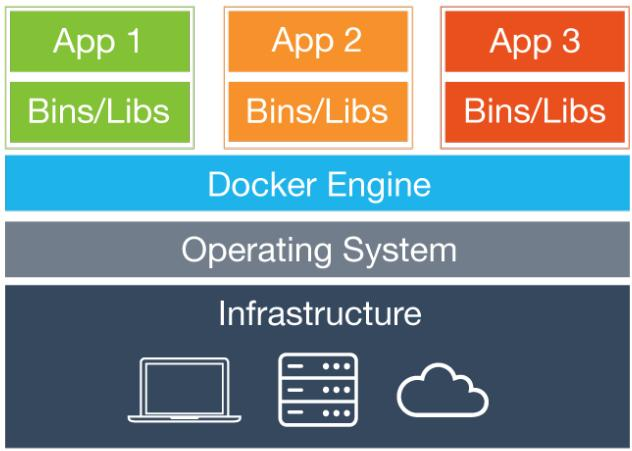
\includegraphics[scale=0.3]{arqdocker}
\end{center}
\legend{Fonte: \citeauthor{docker}, \citeyear{docker}} 
\end{figure}

O Docker tem ganhado fama no mercado, principalmente pelos profissionais de infraestrutura, pois ele tem facilitado o trabalho destas pessoas, pois o trabalho despendido para realizar a instalação de um software foi reduzido, não necessitando mais se preocupar com todas as dependências e ferramentas necessárias para o funcionamento do software, basta apenas se utilizar uma imagem da aplicação e transformá-la em um contêiner.

\subsection{Docker Compose}
O Docker Compose trabalha juntamente com o Docker, ele se caracteriza por definir e executar múltiplos contêineres, pois através do uso de um arquivo que descreve todos os contêineres e configurações necessárias para o funcionamento de uma aplicação por completa, o Docker Compose tem a capacidade de criá-los, reiniciá-los e desligá-los quando necessário, facilitando assim o uso de contêineres.

\section{Tecnologias}
\label{sec:tecnologias}
Mostrar de forma específica cada tecnologia que será empregada
\subsection{Micro Serviços}
Falar sobre

\subsection{Clojure}
Apresentar a linguagem de programação \textit{Clojure} e como ela é empregada no trabalho.

\subsection{Docker e Docker Swarm}
Apresentar o uso de containers \textit{Docker} para encapsular componentes do sistema e \textit{Docker Swarm} para balancear cargas entre containers.

\subsection{Redis}
Mostrar o uso de um \textit{cache} dentro do sistema, sua importância e melhora no desempenho do sistema.

\subsection{Kafka}
Apresentar seu uso para realizar funções em tempo real dentro do sistema, bem como seu funcionamento.

\subsection{MongoDB}
Apresentar as características do banco NoSQL seu uso e diferenças entre um banco SQL, bem como seus pontos positivos.

\subsection{Datomic}
Apresentar uma nova forma de armazenar dados, se utilizando de histórico, sempre mantendo o estado anterior dos dados.

